% !TEX root = ../../semexp-thesis.tex

\section{Exploratory Programming}
\label{sec:background/exp}

\emph{Exploratory programming} is a software engineering practice that promotes a notion of projects where programmers have a rather emergent than upfront understanding of the problem domain~\cite{sandberg1988smalltalk,kery2017exploring,rein2018exploratory}:
for example, they might not know how a new user interface should look and feel like to achieve a good user experience, or they might be unaware of the facilities and limitations that an existing code base or framework provides.
To acquire such knowledge, the exploratory programming practice tightly intertwines reverse engineering, prototyping, and testing in an iterative manner~\cite{taeumel2022pattern}.

\begin{figure}
	\centering
	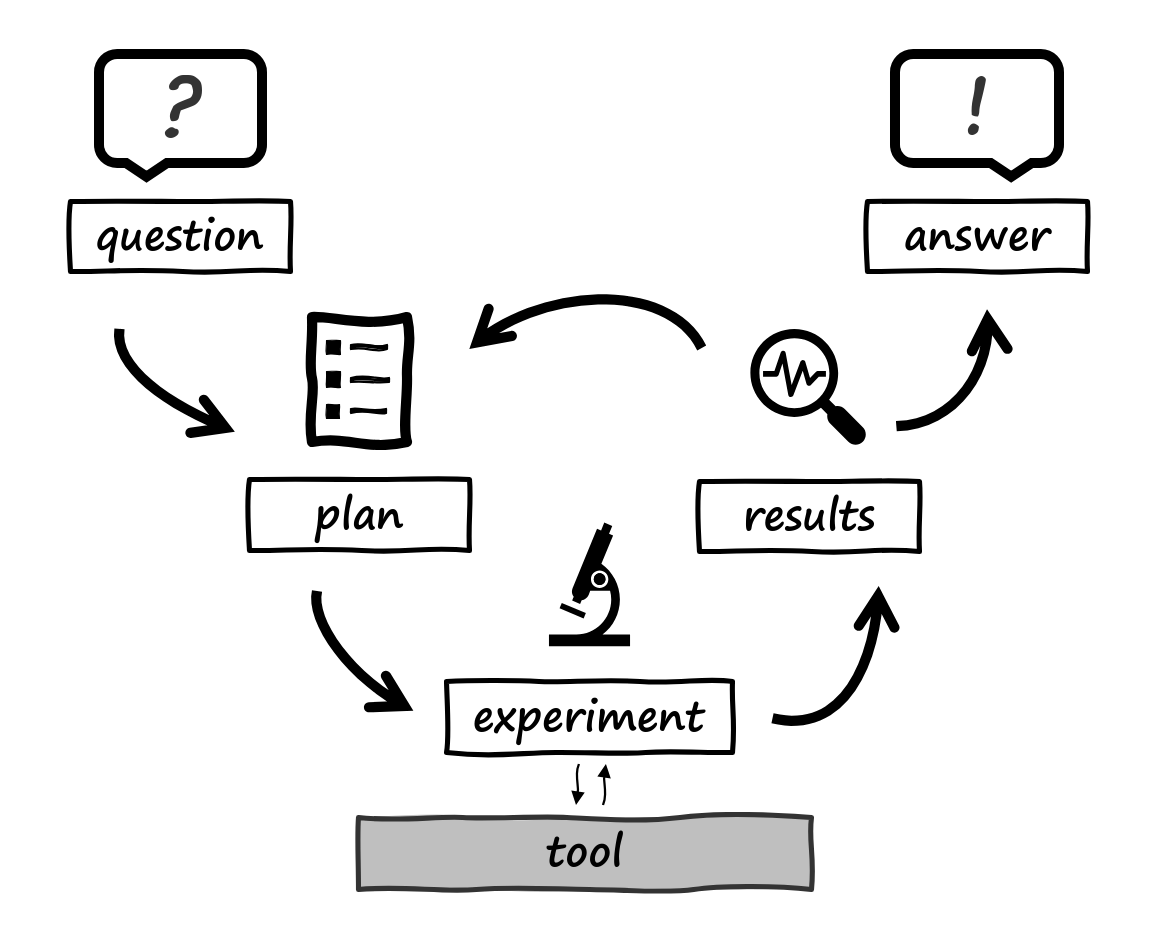
\includegraphics[width=.7\textwidth]{01_exp/simple_process.png}
	% todo: add system below tool?
	\caption[A single \emph{research process} in the \emph{exploratory programming workflow}.]{
		A single research process instance in the exploratory programming workflow.
		Exploratory programmers start with a question about the system.
		To answer the question, they plan one or multiple experiments, execute them by interacting with the system through tools, and observe their results.
		They repeat until they have acquired enough information and then combine them to answer the initial question.
	}
	\label{fig:background/exp/simple_process}
\end{figure}

In our model of an \emph{exploratory programming workflow}, we employ a metaphor from ordinary science:
exploratory programmers are like scientists in the project domain who apply the scientific method and iteratively refine their comprehension of both the problem domain and the solution domain.
To refine their comprehension, they ask questions and find answers to them.
\Cref{fig:background/exp/simple_process} displays a single instance of a \emph{research process} in our exploratory programming workflow model.

Finding answers requires programmers to descend from the conceptual level of the original questions (their \emph{mental model}) into a lower abstraction level where they can dissect questions into their underlying terms, concepts, and technical foundations (the \emph{technical model}).
Here, they interact with the underlying systems by planning, executing, and evaluating a substantial number of \emph{experiments} and repeat until they are able to provide an answer to the original question.
Experiments include a wide range of activities that are aimed at the generation of knowledge:
for example, programmers can research information in the documentation or implementation of a system or related communication platforms; inspect objects of a system at runtime to understand their internal state; run scripts to test interfaces and observe their effect; build and test prototypes; etc.

For nontrivial questions, the research process often spans multiple abstraction levels, as the experiments that programmers plan to answer high-level questions still exhibit an abstraction level that is too high to directly communicate them to the system.
Thus, programmers need to handle abstract experiments as new, subordinate questions and answer them on a lower abstraction level.
This leads to a \emph{hierarchical research process} in which programmers gradually descend into the implementation details of the subjects of questions until they reach the interfaces of the system through which they can execute technical experiments.
\Cref{fig:background/exp/complex_process} displays a complex research process that exploratory programmers walk through when answering a high-level question.

\begin{figure}
	\centering
	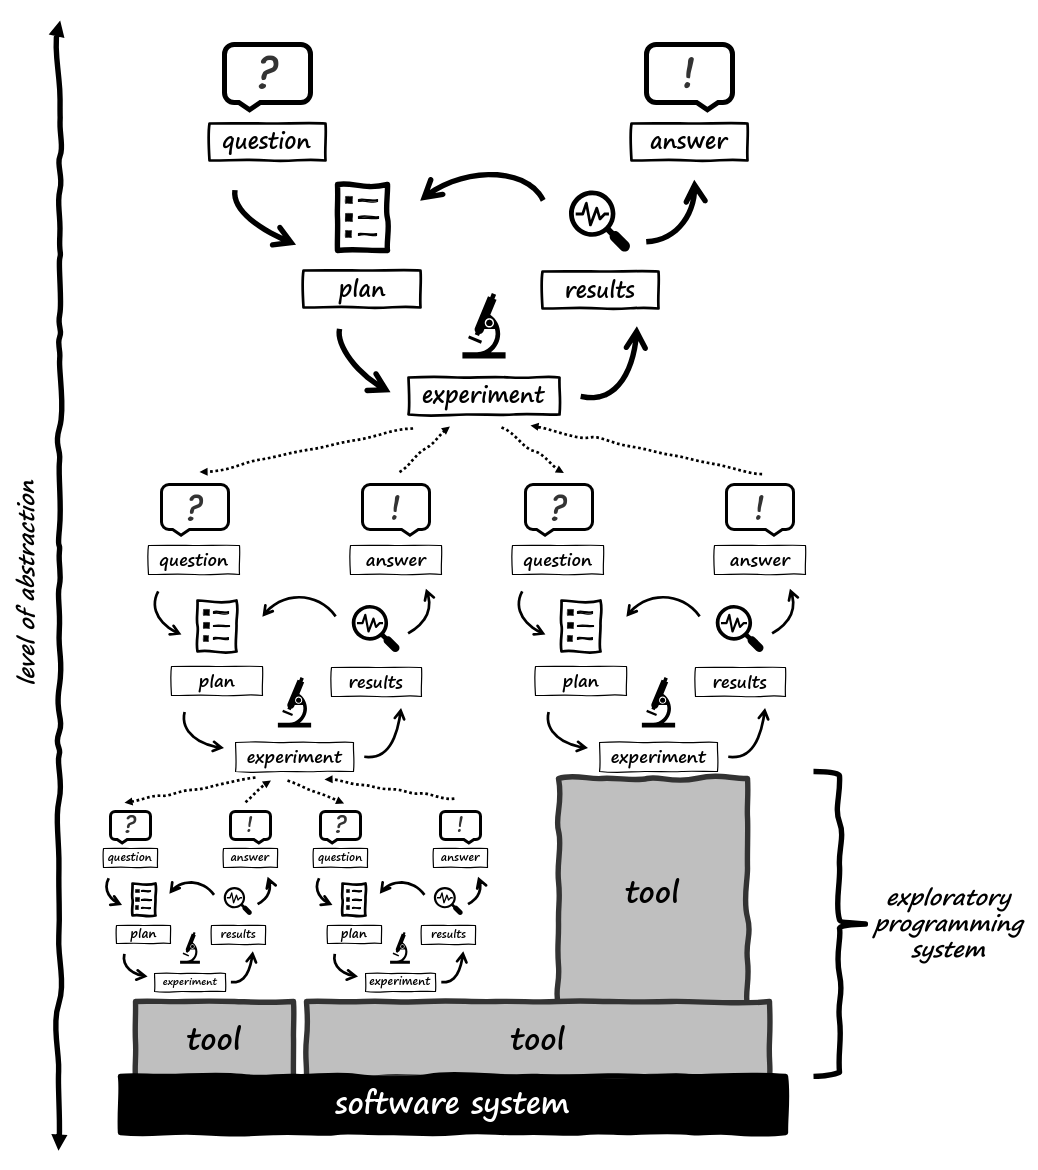
\includegraphics[width=\textwidth]{01_exp/complex_process.png}
	% todo: add interaction arrows between experiments and tools
	\caption[A \emph{hierarchical research process} in the exploratory programming workflow.]{
		A complex, hierarchical research process in the exploratory programming workflow.
		To answer a high-level question about the system, programmers need to bridge multiple levels of abstractions by incrementally breaking down experiments into more concrete questions and answering those until they reach the interfaces of the exploratory programming system.
		The programming system consists of different low-to-medium-level tools for interacting with the software system.
	}
	\label{fig:background/exp/complex_process}
\end{figure}

\begin{example}
	A programmer might wish to design a new user interface (``How could a convenient UI look like?'').
	To answer this question, they plan to experiment with different UI concepts that they want to test through small prototypes (``Let's build a tree-based or pane-based interface and play around with it!'').

	However, to execute these experiments, the programmer needs to perform subordinate research processes in which they conduct further experiments to implement and test single prototypes (``How can I create a tree widget? How can I retrieve the required data? How many interactions are required to navigate through this UI?'').

	Recursively, some of these research processes might yield further experiments that need to be further broken down before they can be communicated to the system (``What classes does this package provide to build widgets? What messages does this class understand? What usage patterns do existing users of this class show?'').
	% todo: maybe concrete fig?
\end{example}
